\documentclass{article}
\usepackage{spconf,amsmath}

% *** MISC UTILITY PACKAGES ***
\usepackage{color}				
\usepackage{url}
\usepackage{hyperref}
\hypersetup{
	colorlinks=true,
	linkcolor=black,
	citecolor=black,
	filecolor=black,
	urlcolor=black
}

% *** GRAPHICS RELATED PACKAGES ***
%
\usepackage[pdftex]{graphicx}

\usepackage{subcaption}
\captionsetup[figure]{name=Fig., labelsep=period} % ICIP2017 template
\captionsetup[table]{name=Table, labelsep=period} % ICIP2017 template
\captionsetup[subfigure]{labelformat=simple}
\renewcommand*{\thesubfigure}{(\alph{subfigure})} % adds parens around subfigure label for clean subreference using \ref{} or \subref{}.
% *** MATH PACKAGES ***
\usepackage{amsfonts}
\usepackage{amsmath}
\usepackage{bm}
\usepackage{amsthm}
\DeclareMathOperator*{\argmin}{argmin}
\DeclareMathOperator{\sinc}{sinc}
\newcommand\undermat[2]{%
	\makebox[0pt][l]{$\smash{\underbrace{\phantom{%
					\begin{matrix}#2 \end{matrix}}}_{\text{$#1$}}}$}#2}
\newtheorem{theorem}{Theorem}


% *** SI UNIT PACKAGE ***
\usepackage{siunitx}
\sisetup{detect-all}

% *** FLOAT PACKAGES ***
\usepackage{subcaption}
\usepackage{multirow}


% *** USEFUL COMMANDS ***
\newcommand{\ie}{\textit{i.e.}}
\newcommand{\etal}{\textit{et al.}}
\newcommand{\vect}[1]{\bm{#1}}
\newcommand{\mat}[1]{\mathsf{#1}}
\newcommand{\ser}[2]{#1^{#2}}
\DeclareMathOperator{\R}{\mathbb{R}}
\theoremstyle{definition}
\newtheorem{defn}{Definition}
% *** TIKZ SETTINGS***
% *** TIKZ PACKAGES ***
\usepackage{xparse}
\usepackage{tikz}
\usetikzlibrary{shapes, arrows.meta, decorations.pathmorphing}
\usetikzlibrary{calc, positioning}
\usetikzlibrary{backgrounds}
\usetikzlibrary{intersections} % provides name path=
\usetikzlibrary{angles} % provides pic angle

\usepackage{etoolbox}

% Tikzset
\tikzset{%
	block/.style = {draw, shape=rectangle, thick, minimum height=2em, minimum width=2em},
	sum/.style = {draw, shape=circle, thick, inner sep=0pt},
	conn/.style={fill, shape=circle, minimum size=0.1cm, inner sep=0, outer sep=0},
	inout/.style={inner sep=0, outer sep=0},
	dot/.style={fill=, shape=circle, minimum size=\pgflinewidth, inner sep=0, outer sep=0},
	param/.style={inner sep=0, outer sep=1pt},
	loosely dotted round/.style={dash pattern=on 0pt off 6\pgflinewidth, line cap=round},
	%	transducer/.style = {shape=rectangle, draw=black, fill=black!20!white, thick, minimum height=0.15cm, minimum width=0.30cm, inner sep=0pt},
	%	my funny rectangle/.style n args={4}{%
	%    rectangle,
	%    draw,
	%    fit={(#1,#3) (#2,#4)}
	%%    append after command={\pgfextra{\let\mainnode=\tikzlastnode}
	%%      node[above right] at (\mainnode.north west) {#3}%
	%%      node[above left] at (\mainnode.north east) {#4}%
	%%      node[below left] at (\mainnode.north west) {#1}%
	%%      node[above left] at (\mainnode.south west) {#2}%
	%%    },
	%  }
}

%\def\td_number{3}

%\newcommand*{\transducer}[4][-1][-2]{\path[draw=black, fill=black!20!white] (#3, #1) rectangle (#4, #2)}

% arg1: lx (optional, default=1)
% arg2: ly (optional, default=2)
% arg3: x_center
% arg4: y_center
%\NewDocumentCommand{\transducer}{ O{-1} O{-2} m }{\path[draw=black, fill=black!20!white] (#3, #1) rectangle (#4, #2)}

\NewDocumentCommand{\rectangle}{ m m }{%
	%\newlength{\Xone}{#1 cm}%\pgfmathparse{#1+1}\pgfmathresult
	\path[draw=black, fill=black!20!white] #1 rectangle #2
}

%\pgfdeclarelayer{bg}    % declare background layer
%\pgfsetlayers{bg,main}  % set the order of the layers (main is the standard layer)

% This bascially automates a \newcommand{<name>}{} to ensure
% that a command with the given <name> does not already exist
\newcommand*{\pgfmathsetnewmacro}[2]{%
	\newcommand*{#1}{}% Error if already defined
	\pgfmathsetmacro{#1}{#2}%
}%

% Transducer commands
\newcommand*{\transducerNumb}{10}
\newcommand*{\transducerWidth}{0.75}
\newcommand*{\transducerHeight}{0.25}
\newcommand*{\transducerInitXPos}{3}
\newcommand*{\transducerXOffset}{1}
\definecolor{transducer-color}{gray}{0.8}
\newcommand*{\transducerLabeled}{9}
\newcommand*{\transducerLabeledBis}{7}

% Measurement commands
\newcommand*{\measurementLength}{6}
\definecolor{measurement-color}{gray}{0.7}

% Insonified domain
\pgfmathsetmacro{\domainXMin}{\transducerInitXPos}
\pgfmathsetmacro{\domainXMax}{12}
\pgfmathsetmacro{\domainZMin}{1}
\pgfmathsetmacro{\domainZLength}{7}
\pgfmathsetmacro{\domainZMax}{\domainZMin+\domainZLength}
\pgfmathsetmacro{\domainDxOffset}{1}
\pgfmathsetmacro{\domainDzOffset}{1}
\definecolor{domain-color}{gray}{0.7}
\definecolor{scatterer-color}{gray}{0}

% Wavefront and time of flight
\definecolor{wavefront-color}{gray}{0.5}

% Axes
\newcommand*{\axesOffset}{1.5}

% Conics
\definecolor{conic-color}{gray}{0}
% 	Ellipse
% http://tex.stackexchange.com/questions/75017/draw-an-ellipse-from-the-two-focus-points-foci-and-the-sum-of-the-distances-fr
\newcommand*{\ellipsebyfoci}[4]{% options (draw, fill, color, etc.), focus pt1, focus pt2, cste
	\path[#1] let \p1=(#2), \p2=(#3), \p3=($(\p1)!.5!(\p2)$)
	in \pgfextra{
		\pgfmathsetmacro{\angle}{atan2(\x2-\x1,\y2-\y1)}
		\pgfmathsetmacro{\distfoci}{veclen(\x2-\x1,\y2-\y1)/1cm} % convert back to cm
		\pgfmathsetmacro{\axeone}{#4/2}
		\pgfmathsetmacro{\axetwo}{sqrt(\axeone^2 - (0.5*\distfoci)^2)}
%		\pgfmathsetmacro{\focal}{veclen(\x2-\x1,\y2-\y1)/2/1cm}
%		\pgfmathsetmacro{\lentotcm}{\focal*2*#4}
%		\pgfmathsetmacro{\axeone}{(\lentotcm - 2 * \focal)/2+\focal}
%		\pgfmathsetmacro{\axetwo}{sqrt((\lentotcm/2)*(\lentotcm/2)-\focal*\focal}
	}
%	(\p3) ellipse[x radius=\axeone cm,y radius=\axetwo cm, rotate=\angle];
	(\p3) ellipse[x radius=\axeone,y radius=\axetwo, rotate={90-\angle}];
%	(\p1) -- node[midway, sloped, above]{\distfoci} (\p2);
}

\name{Adrien~Besson$^{\star}$,
	Dimitris~Perdios$^{\star}$,
	Yves~Wiaux$^{\ast}$,
	Jean-Philippe Thiran$^{\star, \dagger}$\thanks{This work was supported by the UltrasoundToGo RTD project (no. 20NA21\_145911), funded by Nano-Tera.ch.}}% <-this % stops a space

\address{$^{\star}$Signal Processing Laboratory (LTS5),
	Ecole Polytechnique F\'{e}d\'{e}rale de Lausanne, Switzerland\\
	$^{\ast}$Institute of Sensors, Signals and Systems, Heriot-Watt University, UK\\
	$^{\dagger}$Department of Radiology, University Hospital Center and University of Lausanne, Switzerland}%

\begin{document}
\ninept
%
% paper title
% Titles are generally capitalized except for words such as a, an, and, as,
% at, but, by, for, in, nor, of, on, or, the, to and up, which are usually
% not capitalized unless they are the first or last word of the title.
% Linebreaks \\ can be used within to get better formatting as desired.
% Do not put math or special symbols in the title.
\title{Pulse-stream models in time-of-flight imaging}
%
%
% author names and IEEE memberships
% note positions of commas and nonbreaking spaces ( ~ ) LaTeX will not break
% a structure at a ~ so this keeps an author's name from being broken across
% two lines.
% use \thanks{} to gain access to the first footnote area
% a separate \thanks must be used for each paragraph as LaTeX2e's \thanks

% make the title area
\maketitle

% As a general rule, do not put math, special symbols or citations
% in the abstract or keywords.
\begin{abstract}
	This paper considers the problem of reconstructing raw signals from random projections in the context of time-of-flight imaging with an array of sensors. It presents a new signal model, coined as \textit{multi-channel pulse-stream model}, which exploits pulse-stream models and accounts for additional structure induced by inter-sensor dependencies. We propose a sampling theorem and a reconstruction algorithm, based on $\ell_1$-minimization, for signals belonging to such a model. We demonstrate the benefits of the proposed approach by means of numerical simulations and on a real non-destructive-evaluation application where the peak-signal-to-noise-ratio is increased by \SI{3}{\decibel} compared to standard compressed-sensing strategies. 
\end{abstract}

% Note that keywords are not normally used for peerreview papers.
\begin{keywords}%
Compressed sensing, sparsity, array imaging
\end{keywords}






% For peer review papers, you can put extra information on the cover
% page as needed:
% \ifCLASSOPTIONpeerreview
% \begin{center} \bfseries EDICS Category: 3-BBND \end{center}
% \fi
%
% For peerreview papers, this IEEEtran command inserts a page break and
% creates the second title. It will be ignored for other modes.
\maketitle
\section{Introduction}
\label{sec_intro}
\begin{figure}[htb]
	\centering
	\begin{tikzpicture}[%
	scale=\columnwidth/15cm,
	>={Stealth[inset=0pt]},
	thick,
	transducer/.style = {scale=\columnwidth/15cm, shape=rectangle, draw=black, fill=transducer-color, thick, minimum height=\transducerHeight cm, minimum width=\transducerWidth cm, inner sep=0pt},
	measurement/.style = {decorate, decoration=snake, color=measurement-color, thick}
	]
	% Help grid
%	\draw[help lines] (0,0) grid[step=0.5cm] (20, -15);
	
	% Transducers
	\coordinate (pos_td1) at (\transducerInitXPos, {0.5*\transducerHeight});
	\coordinate (xoff_td) at (\transducerXOffset, 0);
	
	\foreach \pt in {1,...,\transducerNumb}
		\node[transducer] (td\pt) at ($ (pos_td1) + \pt*(xoff_td) - (xoff_td) $) {};
	
	% Scatterer
	\pgfmathsetmacro{\scatPointX}{9.6} % use axes_orig
	\pgfmathsetmacro{\scatPointZ}{4.2}

	% http://tex.stackexchange.com/questions/3594/tikz-node-labels-more-below-than-below#3596
%	\node[fill, shape=circle, minimum size=0.1cm, inner sep=0cm, outer sep=0cm, color=scatterer-color, label=below:\textcolor{scatterer-color}{$\left(\vect{r}, \gamma\left(\vect{r}\right)\right)$}] (scatterer_point) at (\scatPointX, -\scatPointZ) {}; % NOT exactly 0.1cm radius..., not exactly the correct "below" distance
	\node[fill, shape=circle, minimum size=0.1cm, inner sep=0cm, outer sep=0cm, color=scatterer-color] (scatterer_point) at (\scatPointX, -\scatPointZ) {};
	\fill[color=scatterer-color] (scatterer_point) circle[radius=0.1] node[below]{$\vect{r}^k$};
	
	% Measurements
%	\pgfmathsetmacro{\pt}{7}
%	\pgfmathsetmacro{\tdPosX}{\transducerInitXPos+(\pt-1)*\transducerXOffset}
%	\pgfmathsetmacro{\rForward}{\scatPointZ} % z
%	\pgfmathsetmacro{\rBackward}{sqrt((\scatPointX - \tdPosX)^2 + \scatPointZ^2)}
%	\pgfmathsetmacro{\rTot}{\rForward+\rBackward}
%	\pgfmathsetmacro{\tPulseCenter}{\rTot/1 - 11.5}
%	
%	\pgfmathsetmacro{\tStart}{\measurementLength - \tPulseCenter - 1/2}
%	\pgfmathsetmacro{\tEnd}{\tStart + 1}
%	\draw[domain=0:\tStart, thick, smooth, variable=\t, red] plot ({\tdPosX+0*\t}, {\t+\transducerHeight});
%	\draw[domain=0:1, thick, smooth, variable=\t, red]  plot ({\tdPosX + 0.5*(1-cos((2*pi*\t) r))*0.4*\transducerWidth*sin(3*2*pi*(\t) r)},{\transducerHeight+\tStart+\t});
%	\draw[domain=\tEnd:\measurementLength, thick, smooth, variable=\t, red] plot ({\tdPosX+0*\t}, {\t+\transducerHeight});
%	%	\node[above] at (\tdPosX, \measurementLength + \transducerHeight) {\rotatebox{90}{\textcolor{blue}{\tPulseCenter}}};
	
	\begin{scope}[on background layer]
	\foreach \pt in {1,...,\transducerNumb}
	{
		\pgfmathsetmacro{\tdPosX}{\transducerInitXPos+(\pt-1)*\transducerXOffset}
		\pgfmathsetmacro{\rForward}{\scatPointZ} % z
		\pgfmathsetmacro{\rBackward}{sqrt((\scatPointX - \tdPosX)^2 + \scatPointZ^2)}
		\pgfmathsetmacro{\rTot}{\rForward+\rBackward}
%		\pgfmathsetmacro{\tPulseCenter}{\rTot/1 - 11.5}
		\pgfmathsetmacro{\tPulseCenter}{\rTot/1 - 7.5}
		
		\pgfmathsetmacro{\tStart}{\measurementLength - \tPulseCenter - 1/2}
		\pgfmathsetmacro{\tEnd}{\tStart + 1}
		\draw[domain=0:\tStart, thick, smooth, variable=\t, measurement-color] plot ({\tdPosX+0*\t}, {\t+\transducerHeight});
		\draw[domain=0:1, thick, smooth, variable=\t, measurement-color]  plot ({\tdPosX + 0.5*(1-cos((2*pi*\t) r))*0.4*\transducerWidth*sin(3*2*pi*(\t) r)},{\transducerHeight+\tStart+\t});
		\draw[domain=\tEnd:\measurementLength, thick, smooth, variable=\t, measurement-color] plot ({\tdPosX+0*\t}, {\t+\transducerHeight});
%		\node[above] at (\tdPosX, \measurementLength + \transducerHeight) {\rotatebox{90}{\textcolor{blue}{\tPulseCenter}}};
		
		% Measurement label
%		\draw[] (\tdPosX, \transducerHeight) -- node[midway, sloped, below]{$m\left(\vect{r}_{ts}^i, t\right)$} (\tdPosX, {\tStart+\transducerHeight});
		\ifdefstrequal{\pt}{\transducerLabeled}{%
			\fill[color=measurement-color] (\tdPosX, {0.5*\tStart+0.5*\tEnd+\transducerHeight}) circle[radius=0] node[below left]{\rotatebox{90}{$m\left(\vect{p}^i, t\right)$}};
			% COULD USE \path without option for an invisible path
		}{}
		
	}
	\end{scope}
	
	% Labels for transducer and measurement
	\pgfmathsetmacro{\tdPosX}{\transducerInitXPos+(\transducerLabeled-1)*\transducerXOffset}
	\node[above] at (td\transducerLabeled) {$\vect{p}^i$};
	
	\pgfmathsetmacro{\tdPosX}{\transducerInitXPos+(\transducerLabeledBis-1)*\transducerXOffset}
	\node[above] at (td\transducerLabeledBis) {$\vect{p}^j$};
	
%	\node[above] at (\tdPosX, \measurementLength + \transducerHeight) {\rotatebox{90}{\textcolor{measurement-color}{$m\left(\vect{r}_{ts}^i, t\right)$}}};
	
	
	% Axes
	\pgfmathsetmacro{\vertAxisX}{\transducerInitXPos - \axesOffset}
	\pgfmathsetmacro{\transducerLength}{(\transducerNumb-1)*\transducerXOffset}
	\coordinate (axes_orig) at (\vertAxisX, 0);
	\coordinate (x_axis_end) at ({\transducerInitXPos + \transducerLength + \axesOffset}, 0);
%	\coordinate (z_axis_end) at (\vertAxisX, {-\scatPointZ - \axesOffset});
	\coordinate (z_axis_end) at (\vertAxisX, {-\scatPointZ - 0.5*\axesOffset});
	\coordinate (t_axis_start) at (\vertAxisX, \transducerHeight + \measurementLength);
	\coordinate (t_axis_end) at (\vertAxisX, \transducerHeight + \axesOffset);
	
	\draw[<->] (x_axis_end) node[right] {$x$} -- (axes_orig) -- (z_axis_end) node[below] {$z$};
	\draw[->] (t_axis_start) -- (t_axis_end) node[below] {$t$};

	% Plane wave: Wavefront and transmit time of flight
	\pgfmathsetmacro{\thetaPW}{15} % degree
	\pgfmathsetmacro{\thetaLabXOffset}{2.2}
	\pgfmathsetmacro{\PWaveFrontStartX}{\transducerInitXPos}
	\pgfmathsetmacro{\PWaveFrontStartZ}{\transducerHeight}
	\pgfmathsetmacro{\PWaveFrontEndX}{\transducerInitXPos+\transducerLength}
	\pgfmathsetmacro{\PWaveFrontEndZ}{\transducerHeight+sin(\thetaPW)*\transducerLength}
	\coordinate (pw_wavefront_start) at (\PWaveFrontStartX, \PWaveFrontStartZ);
	\coordinate (pw_wavefront_end) at (\PWaveFrontEndX, \PWaveFrontEndZ);
	\coordinate (pw_wavefront_scat_proj) at ($(pw_wavefront_start)!(scatterer_point)!(pw_wavefront_end)$);
	
	%	Transmit wavefront
	\begin{scope}[on background layer]
		\draw[dashed, wavefront-color, thick, name path=pw_wavefront_path] (pw_wavefront_start) -- (pw_wavefront_end);
		%TODO: use clip on an extended path line
	\end{scope}
%	%		Angle
%	\begin{scope}[on background layer]
%		\draw[wavefront-color, thin] ({\PWaveFrontStartX+\thetaLabXOffset},{\PWaveFrontStartZ}) arc[start angle=0, end angle=\thetaPW, radius=\thetaLabXOffset] node[midway, right]{$\theta$};
%	\end{scope}
	
	% 		Wavefront label
	\path[name path=data_right_limit_path] ({\transducerInitXPos+\transducerLength}, 0) -- ({\transducerInitXPos+\transducerLength}, {\transducerHeight+\measurementLength});
	\fill[name intersections={of=pw_wavefront_path and data_right_limit_path, by = pw_wavefront_label_point}] (pw_wavefront_label_point) circle[radius=0] node[right, align=center, wavefront-color]{``wavefront''}; % specificying the key align= allows to add newlines
	
	%	Transmit time of flight
	\draw[->, wavefront-color] (pw_wavefront_scat_proj) -- node[midway, sloped, below] {$t_{Tx}\left(\vect{r}^k\right)$} (scatterer_point);
	
%	% Diverging wave: Wavefront and transmit time of flight
%	\pgfmathsetmacro{\DWVirtualPointX}{\transducerInitXPos + 3}
%	\pgfmathsetmacro{\DWVirtualPointZ}{1.2*\measurementLength + \transducerHeight}
%	\pgfmathsetmacro{\DWBetaAngleRadius}{0.35cm}
%	
%	%	Virtual point
%	\node[fill, shape=circle, minimum size=0.1cm, inner sep=0cm, outer sep=0cm, color=wavefront-color] (dw_virtual_point) at (\DWVirtualPointX, \DWVirtualPointZ) {};
%	\fill[color=wavefront-color] (dw_virtual_point) circle[radius=0] node[above]{$\vect{r}^k_n$};
%	
%	%	Wavefront
%	\begin{scope}[on background layer]
%%		\clip (\transducerInitXPos, \transducerHeight) rectangle ({\transducerInitXPos+\transducerLength}, {\transducerHeight, \measurementLength});
%		\begin{scope} % just for the clip
%			\clip (\transducerInitXPos, \transducerHeight) rectangle ({\transducerInitXPos+\transducerLength}, {\transducerHeight+\measurementLength});
%%		\path[draw, thick, wavefront-color, name path=dw_wavefront_path] (dw_virtual_point) circle [radius={\DWVirtualPointZ-\transducerHeight}];
%			\draw[dashed, thick, wavefront-color, name path=dw_wavefront_path] (dw_virtual_point) circle [radius={\DWVirtualPointZ-\transducerHeight}];
%		\end{scope}
%	\end{scope}
%	
%	% 		Wavefront label
%	\path[name path=data_right_limit_path] ({\transducerInitXPos+\transducerLength}, 0) -- ({\transducerInitXPos+\transducerLength}, {\transducerHeight+\measurementLength});
%	\fill[name intersections={of=dw_wavefront_path and data_right_limit_path, by = dw_wavefront_label_point}] (dw_wavefront_label_point) circle[radius=0] node[right, align=center, wavefront-color]{``wavefront''}; % specificying the key align= allows to add newlines
%	
%	%	Intersection on the circular wavefront
%	\path[name path=dw_virtual_point_to_scatterer] (dw_virtual_point) -- (scatterer_point);
%	
%	% 	Transmit time of flight
%	\fill[name intersections={of=dw_wavefront_path and dw_virtual_point_to_scatterer, by = dw_point_on_wavefront}] (dw_point_on_wavefront) circle[radius=0];
%%	\draw[-, wavefront-color] [name intersections={of=dw_wavefront_path and dw_virtual_point_to_scatterer, by = dw_point_on_wavefront}] (dw_virtual_point) -- (dw_point_on_wavefront);
%	\draw[dotted, wavefront-color] (dw_virtual_point) -- (dw_point_on_wavefront);
%	\draw[->, wavefront-color](dw_point_on_wavefront) -- node[midway, sloped, below] {$t_{Tx}\left(\vect{r}^k\right)$} (scatterer_point);
%	\begin{scope}[on background layer]
%		\path[name path=transducer_height_path] (\vertAxisX, \transducerHeight) -- ({\transducerInitXPos+\transducerLength+\axesOffset}, \transducerHeight);
%		%	Angle
%		\fill[red, name intersections={of=transducer_height_path and dw_virtual_point_to_scatterer, by = dw_beta_base_point}] (dw_beta_base_point) circle[radius=0cm];
%		\pic[pic text=$\beta$, draw, wavefront-color, thin, angle radius=\DWBetaAngleRadius, angle eccentricity=1.4] {angle= dw_virtual_point--dw_beta_base_point--td1};
%	\end{scope}
%
%	
	% Receive time for flight
	\draw[->, wavefront-color] (scatterer_point) -- node[midway, sloped, below] {$\frac{\|\vect{r}^k-\vect{p}^i\|_2}{c}$} (td\transducerLabeled.south);
%	
%	% 1-D conic (ellipse)
%	\coordinate (dw_ellipse_focus1) at (dw_virtual_point);
%	\coordinate (dw_ellipse_focus2) at (td\transducerLabeled);
%	\begin{scope} % just for the clip
%		\clip (\transducerInitXPos, 0) rectangle ({\transducerInitXPos+\transducerLength}, -\domainZMax);
%		\ellipsebyfoci{draw, conic-color, name path=dw_conic_path}{dw_ellipse_focus1}{dw_ellipse_focus2}{16.5}
%	\end{scope}
%	%	Conic label
%	\newcommand*{\conicTextLabel}{``ellipse''}
%	\newcommand*{\conicMathLabel}{$\left[
%		x\left(\alpha\right), z\left(\alpha\right)\right]^T$}
%	\pgfmathsetmacro{\vertGridX}{\transducerInitXPos+9*\transducerXOffset}
%	\path[name path=domain_vert_path] (\vertGridX, 0) -- (\vertGridX, -\domainZMax);
%	\fill[name intersections={of=dw_conic_path and domain_vert_path, by = dw_conic_label_point}] (dw_conic_label_point) circle[radius=0] node[right, align=center, conic-color]{\conicTextLabel}; % specificying the key align= allows to add newlines
%	
%	% Insonified domain (i.e. Grid)
%	% http://tex.stackexchange.com/questions/45808/tikz-grid-lines
%	\begin{scope}[on background layer]
%		\draw[step=1, very thin, color=domain-color] (\domainXMin, -\domainZMin) grid (\domainXMax, -\domainZMax);
%	\end{scope}
%	
%	% 	Discretization
%	\pgfmathsetmacro{\discretizedPointLabeledNumb}{3}
%%	\newcommand*{\discretizedPointMathLabel}{$\left[
%%		x\left(\alpha^p\right), z\left(\alpha^p\right)\right]^T$}
%	\newcommand*{\discretizedPointMathLabel}{$\vect{r}\left(\alpha^p\right)$}
%	%		TODO: set a gridNumb
%	\foreach \gridVert in {1,...,\transducerNumb}
%	{
%		\pgfmathsetmacro{\vertGridX}{\domainXMin+(\gridVert-1)*\domainDxOffset}
%		\path[name path=domain_vert_path] (\vertGridX, -\domainZMin) -- (\vertGridX, -\domainZMax);
%		\fill[name intersections={of=dw_conic_path and domain_vert_path, by = discretized_conic_point}] (discretized_conic_point) circle[radius=0.1];
%		
%		\ifdefstrequal{\gridVert}{\discretizedPointLabeledNumb}{%
%			\fill (discretized_conic_point) circle[radius=0] node[above right]{\discretizedPointMathLabel};
%			% COULD USE \path without option for an invisible path
%		}{}
%	}
%	
%	%	Grid spacing
	\newcommand*{\spacingLabelOffset}{0pt}
%	\pgfmathsetmacro{\domainDxIndexX}{8} % 1 - 10
%	\pgfmathsetmacro{\domainDxIndexZ}{8} % 1 - 8
%	\pgfmathsetmacro{\domainDzIndexX}{10} % 1 - 10
%	\pgfmathsetmacro{\domainDzIndexZ}{6} % 1 - 8
%	\pgfmathsetmacro{\domainDxOneX}{\domainXMin+(\domainDxIndexX-1)*\domainDxOffset}
%	\pgfmathsetmacro{\domainDxTwoX}{\domainXMin+(\domainDxIndexX)*\domainDxOffset}
%	\pgfmathsetmacro{\domainDxOneZ}{-\domainZMin-(\domainDxIndexZ-1)*\domainDzOffset}
%	\pgfmathsetmacro{\domainDxTwoZ}{-\domainZMin-(\domainDxIndexZ-1)*\domainDzOffset}
%	\pgfmathsetmacro{\domainDzOneX}{\domainXMin+(\domainDzIndexX-1)*\domainDzOffset}
%	\pgfmathsetmacro{\domainDzTwoX}{\domainXMin+(\domainDzIndexX-1)*\domainDzOffset}
%	\pgfmathsetmacro{\domainDzOneZ}{-\domainZMin-(\domainDzIndexZ-1)*\domainDzOffset}
%	\pgfmathsetmacro{\domainDzTwoZ}{-\domainZMin-(\domainDzIndexZ)*\domainDzOffset}
%%	\fill[red] (\domainDxOneX, \domainDxOneZ) circle[radius=0.1];
%%	\fill[blue] (\domainDxTwoX, \domainDxTwoZ) circle[radius=0.1];
%%	\fill[red] (\domainDzOneX, \domainDzOneZ) circle[radius=0.1];
%%	\fill[blue] (\domainDzTwoX, \domainDzTwoZ) circle[radius=0.1];
%	\coordinate (domain_dx_one) at (\domainDxOneX, \domainDxOneZ);
%	\coordinate (domain_dx_two) at (\domainDxTwoX, \domainDxTwoZ);
%	\coordinate (domain_dz_one) at (\domainDzOneX, \domainDzOneZ);
%	\coordinate (domain_dz_two) at (\domainDzTwoX, \domainDzTwoZ);
%	\draw[|-|, thin] ($ (domain_dx_one) - (0, \spacingLabelOffset) $) -- node[below] {$\Delta x$} ($ (domain_dx_two) - (0, \spacingLabelOffset) $);
%	\draw[|-|, thin] ($ (domain_dz_two) + (\spacingLabelOffset, 0) $) -- node[midway, sloped, below] {$\Delta z$} ($ (domain_dz_one) + (\spacingLabelOffset, 0) $);
%	
	%	Inter-element spacing
	\pgfmathsetmacro{\transducerDxiOne}{\transducerLabeled}
	\pgfmathsetmacro{\transducerDxiTwo}{\transducerLabeledBis}
%	\draw[|-|, thin] ($ (td\transducerDxiOne.south) - (0, \spacingLabelOffset) $) -- node[below] {$\Delta x_{ij}$} ($ (td\transducerDxiTwo.south) - (0, \spacingLabelOffset) $);
	\draw[<->, thin] ($ (td\transducerDxiOne) - (0, \spacingLabelOffset) $) -- node[below] {$\Delta _{ij}$} ($ (td\transducerDxiTwo) - (0, \spacingLabelOffset) $);
%	
%	
	\end{tikzpicture}
	\caption{Considered time-of-flight imaging configuration.}
	\label{fig_pulse_echo}
\end{figure}
%Pulse-echo ultrasound~(US) imaging is based on the transmission of short acoustic pulses through the human body. When such pulses encounter medium inhomogeneities, part of their energy is reflected back to the array of transducer-elements. The received signals, denoted as element-raw data, consist of backscattered echoes from the medium. Ultrafast US imaging is one specific modality of pulse-echo imaging which exploits the transmission of plane waves~(PW) or diverging waves in order to insonify the whole medium at once~\cite{Tanter_UFFC_2014}. Formally, let us assume that the transducer array is made of $N_{el}$ elements, positioned at $\left(\ser{\vect{r}_{ts}}{p}\right)_{p=1}^{N_{el}}$, as described on Figure~\ref{fig_pulse_echo}. Let us also consider that the medium is made of $K$ point-scatterers positioned at $\left(\vect{r}^k\right)_{k=1}^K$. The signal $m_{p} \left(t\right)$ received at the $p$-th element can be expressed as~\cite{Chernyakova2014, Tur_TSP_2012}:
%\begin{equation}
%\label{eq_raw_data_ultrafast}
%m_{p} \left(t\right) = \sum \limits_{k=1}^{K} a_k h\left(t - \ser{t_p}{k}\right), 
%\end{equation}
%where $a_k$ and $\ser{t_p}{k}$ are the amplitude and delay of the $k$-th point-scatterer and $h\left(t\right)$ is the pulse. In the remainder of the paper, we will consider that the pulse is known and that it can be written as $h\left(t\right) = \left(e \ast h_{ea} \ast h_{ae}\right)\left(t\right)$, where $e\left(t\right)$ is the excitation signal, $h_{ea}\left(t\right)$ is the electro-acoustical impulse response of the transducer elementand $h_{ae}\left(t\right)$ is the acousto-electrical impulse response of the transducer element~\cite{Jensen_UFFC_1992}.

%In the case of US imaging, it is possible to relate the time instant $\ser{t_p}{k}$ to the positions of the point-scatterer~$\ser{\vect{r}}{k}$ and the transducer element~$\ser{\vect{r}_{ts}}{p}$ using the following relationship~\cite{montaldo_uffc_2014}:
%\begin{equation}
%\label{eq_usdelay}
%\ser{t_p}{k} = t_{Tx}\left(\vect{r}^k\right) + t_{Rx}\left(\vect{r}^k, \ser{\vect{r}_{ts}}{p}\right),
%\end{equation}
%where $t_{Tx}\left(\vect{r}^k\right)$ is the propagation delay in transmit ~\cite{montaldo_uffc_2014, Papadacci_UFFC_2014}, and $t_{Rx}\left(\vect{r}^k, \ser{\vect{r}_{ts}}{p}\right)~=~\frac{\|\vect{r}^k - \ser{\vect{r}_{ts}}{p}\|_2}{c}$ is the propagation delay in receive, as described on Figure~\ref{fig_pulse_echo}.

The notion of \textit{pulse stream} has been introduced by Hedge and Baraniuk~\cite{Hedge_TSP_2011} and designates signals that can be expressed as a convolution between a $K$-sparse spike train and a $F$-sparse impulse response. 
%Two main approaches for recovery of pulse-stream signals have been studied. 
%
%The first approach models the pulse stream using the finite rate of innovation~(FRI) framework, which defines sampling theorems and kernels for impulse signals~\cite{Vetterli_TSP_2002}. 
%Indeed, pulse streams can be seen as parametric signals, entirely defined by the amplitudes and delays of the spike train and one may be able to recover the pulse streams with only $2K$ samples. 
%%Tur~\etal{}~\cite{Tur_TSP_2012} as well as Chernyakova~\etal{}~\cite{Chernyakova2014} have applied this framework to US imaging, leading to significant data-rate reduction.
%
%The second approach, which is of interest in this work, exploits sparse representations in the context of the compressed-sensing~(CS) framework~\cite{Candes_SPM_2008}. Indeed, pulse streams are $K$-sparse in the dictionary made of circular shifts of the impulse response~\cite{Naini_ICASSP_2009}. Thus, one may perfectly recover pulse streams from few samples using convex optimization algorithms or greedy approaches~\cite{Hedge_TSP_2011, Naini_ICASSP_2009, Tsagkatakis_ICASSP_2014}.

Formally, let us consider a pulse stream $\vect{z} \in \mathbb{R}^N$, such that $\vect{z} = \vect{h} \ast \vect{s}$ with $\vect{s} \in \mathbb{R}^N$ the $K$-sparse spike train and $\vect{h} \in \mathbb{R}^N$ the $F$-sparse impulse response. 
The following definition holds:
\begin{defn}[Definition 2 of \cite{Hedge_TSP_2011}]	
The pulse-stream model is defined as follows:
\begin{equation}
\label{eq_pulse_stream_model}
\mathcal{M}^z_{K,F}:=\left\lbrace \vect{z} \in \mathbb{R}^N: \vect{z} = \vect{s} \ast \vect{h} \; | \; \vect{s} \in \mathcal{M}_K \textnormal{ and } \vect{h} \in \mathcal{M}_F \right \rbrace,
\end{equation}
where $\mathcal{M}_K \subset \mathbb{R}^N$ and $\mathcal{M}_F \subset \mathbb{R}^N$ are restricted unions of $L_K$ $K$-dimensional and $L_F$ $F$-dimensional canonical subspaces, respectively.
\end{defn} 

For signals belonging to the pulse-stream model $\mathcal{M}^z_{K,F}$, Hedge and Baraniuk~\cite{Hedge_TSP_2011} have derived a sampling theorem where the number of measurements necessary for perfect reconstruction scales linearly with $K + F$ instead of $KF$~(standard CS). 
In this work, we propose to extend this model to time-of-flight imaging with an array of sensor elements, whose configuration is described on Fig.~\ref{fig_pulse_echo}. 
The sensing process is divided into a transmit phase where one or several emitters are used to send a pulsed-wave in the medium, and a receive phase where the sensors are used to acquire the response of the medium to the previously transmitted pulsed wave. 
Such a configuration covers a wide range of applications such as medical ultrasound imaging, non-destructive evaluation, seismic imaging, sonar, lidar and synthetic aperture radar imaging.

Formally, let us assume that the array is made of $N_{el}$ sensors, positioned at $\left(\vect{p}^i\right)_{i=1}^{N_{el}}$, as described on Fig.~\ref{fig_pulse_echo}. 
Let us also consider that the medium is made of $K$ targets positioned at $\left(\vect{r}^k\right)_{k=1}^K$. The signal $m_{i} \left(t\right)$ received at the $i$-th sensor can be expressed as:
\begin{equation}
\label{eq_raw_data}
m_{i} \left(t\right) = \sum \limits_{k=1}^{K} a_k h\left(t - t_i^k\right), 
\end{equation}
where $a_k$ and $t_i^k$ are the amplitude and delay associated with the $k$-th target and $h\left(t\right)$ is the received pulse, supposed to be known in the remainder of the paper. 
The delay associated with the $k$-th target depends on its relative position with respect to the $i$-th sensor and can be expressed as follows:
\begin{equation}
\label{eq_usdelay}
t_i^k = t_{Tx}\left(\vect{r}^k\right) + \frac{\|\vect{r}^k -  \vect{p}^i \|_2}{c},
\end{equation}
where $c$ denotes the wave velocity in the medium, supposed to be constant, and $t_{Tx}\left(\vect{r}^k\right)$ is the transmit delay which depends on the transmit settings. Such model have been extensively used in medical ultrasound imaging~\cite{Chernyakova2014, Tur_TSP_2012, Bendory_TSP_2016}, non-destructive testing~\cite{Carcreff_UFFC_2014} and radar imaging~\cite{Ilan_TSP_2014, Baraniuk2007}. 

Starting from Equation~\eqref{eq_raw_data}, we consider inter-sensor dependencies in order to derive an additional structure of the array signals. 
This structure, expressed as restrictions on the possible support of the array signals, leads us to define a new model, denoted as \textit{multi-channel pulse stream model}, from which we present a sampling theorem and a recovery algorithm.

The remainder of the paper is organized as follows. 
In Section~\ref{sec_pulsestreams_US}, the signal model is presented, with the corresponding sampling theorem and recovery algorithm. 
Section~\ref{sec_exp} presents results on synthetic pulse streams as well as on real non-destructive evaluation signals. Concluding remarks are given in Section~\ref{sec_concl}.
\section{Pulse streams in array imaging}
\label{sec_pulsestreams_US}
\subsection{Signal recovery from the pulse-stream model}
\label{subsec_US_pulsestream}
From Equation~\eqref{eq_raw_data}, one may express the signal $m_i\left(t\right)$ as $m_i\left(t\right) = \left(s_i \ast h\right)\left(t\right)$, where $h\left(t\right)$ is the pulse and 
\begin{equation}
 s_i \left(t\right) = \sum \limits_{k=1}^{K} a_k \delta\left(t - \ser{t_i}{k}\right).
\end{equation} 
Let us consider that the signal $m_i \left(t\right)$ is sampled at a rate $f_s$, leading to $N$ samples $ m_i \left(\ser{t}{j}\right)$, with $\ser{t}{j}= \ser{t}{0} + j/f_s$ for $j \in \left\lbrace 1,\dots,N \right\rbrace$.

The vector $\vect{m}_i = \left[m_i\left(\ser{t}{1}\right),\dots,m_i\left(\ser{t}{N}\right)\right]^T \in \mathbb{R}^N$ belongs to the pulse-stream model $\mathcal{M}^z_{K,F}$ where $F$ denotes the size of the support of $\vect{h} \in \mathbb{R}^N$, supposed to be small compared to $N$, and $K$ the number of point scatterers.

Thus, one may be able to sample array signals at a rate dictated by Hedge and Baraniuk~\cite{Hedge_TSP_2011} while ensuring a perfect recovery using either model-based greedy approaches~\cite{Baraniuk2010} or $\ell_1$-minimization~\cite{candes11}. 
In the proposed work, we have decided to focus on the latter. Since the pulse is supposed to be known, the following convex problem can be solved to retrieve $\vect{m}_i \in \mathbb{R}^M$ from noisy measurements $\vect{y} = \mathsf{\Phi} \vect{m}_i + \vect{n}$, with $\mathsf{\Phi} \in \mathbb{R}^{M \times N}$ a Gaussian \textit{i.i.d.} matrix:
\begin{equation}
\label{eq_l1_BPDN}
\min_{\bar{\vect{s}}}\|\bar{\vect{s}}\|_{1}
\textnormal{ subject to }\| \bm{y}-\mat{\Phi H}\bar{\vect{s}}\|_{2}\leq\epsilon,
\end{equation}
where $\mat{H}$ is a circulant matrix which contains time-shifted replicas of the pulse, $\vect{s}$ is a $K$-sparse vector and $\epsilon \in \mathbb{R}_{+}$.
\subsection{Multi-channel pulse-stream model}
\label{subsec_US_multiplechannels}
The model described in Section~\ref{subsec_US_pulsestream} is suited to single channel reconstructions. 
However, such a model does not account for inter-channel dependencies, which are self-evident in the proposed configuration~(see Fig.~\ref{fig_pulse_echo}). 
By taking into account the dependencies, one may be able to decrease the number of measurements required to reconstruct array signals.
The following theorem precises the way the dependencies between two channels may be expressed.
\begin{theorem}[Two-channel scenario]
\label{th_2sens_subspace}
The support $\sigma \left(\vect{s}_i\right)$ of the spike train $\vect{s}_i$ corresponding to the sensor located at a distance $\Delta_{ij}$ from the sensor $j$, whose spike train is $\vect{s}_j$, has the following property:
	\begin{equation*}
		\sigma \left(\vect{s}_i\right) \subset S_{ij},
	\end{equation*}
	where $S_{ij} := \bigcup \limits_{k=1}^K \ser{\Omega_k}{ij}$ is a union of $2 D_{ij}$-dimensional subspaces $\ser{\Omega_k}{ij}$ defined by: 
	\begin{equation*}
		\ser{\Omega_k}{ij} := \left \lbrace \left \lbrace k - D_{ij},\dots, k+ D_{ij} \right\rbrace, \; k \in \sigma \left(\vect{s}_{j}\right) \right\rbrace,
	\end{equation*}
	where $D_{ij}=\lceil f_s \Delta_{ij}/ c  \rceil$. 
\end{theorem}
In the above theorem, $\lceil.\rceil$ designates the round value.
\begin{proof}
	Let us suppose that $s_j \left(t\right) = \sum_{k=1}^{K} a_k \delta \left(t - \ser{t_j}{k}\right)$ and $s_i \left(t\right) = \sum_{k=1}^{K} a_k \delta \left(t - \ser{t_i}{k}\right)$. From Equation~\eqref{eq_usdelay}, one may deduce the following:
	\begin{align*}
	\ser{t_j}{k} &= t_{Tx}\left(\vect{r}^k\right) + \frac{\|\vect{r}^k - \vect{p}^j \|_2}{c}\\
	&\leq  t_{Tx}\left(\vect{r}^k\right) + \frac{\|\vect{r}^k - \vect{p}^i \|_2}{c} + \frac{\Delta_{ij}}{c}\\
	&\leq \ser{t_i}{k} + \frac{\Delta_{ij}}{c}.
	\end{align*}
	Reversely, one can deduce that $\ser{t_j}{k} \geq \ser{t_i}{k} - \frac{\Delta_{ij}}{c}$, which leads to $\ser{t_i}{k} \in \left[\ser{t_j}{k} -\frac{\Delta_{ij}}{c}, \ser{t_j}{k} +\frac{\Delta_{ij}}{c}\right]$. Thus, by simple multiplication with $f_s$, one may deduce that:
	\begin{equation}
	\label{eq_1_support_x_xj}
		\forall l \in \sigma\left(\vect{s}_i\right), \exists p \in \sigma \left(\vect{s}_j\right) \; | \; l \in \left\lbrace p-D_{ij},\dots,p+D_{ij}\right\rbrace,
	\end{equation}
	where $D_{ij}~=~\lceil f_s \Delta_{ij}/ c  \rceil$. Generalizing Equation~\eqref{eq_1_support_x_xj} to the support of $\sigma\left(\vect{s}_i\right)$, one may retrieve the result of Theorem~\ref{th_2sens_subspace}.
\end{proof}
Theorem~\ref{th_2sens_subspace} states that the support of $\vect{s}_i$ is a union of $K$ \num{2}$D_{ij}$-dimensional subspaces located around the support of the signal received at sensor $j$. The dimension of each subspace depends on the distance between the sensors. 

We can go further than the two-channel scenario by considering that we have prior knowledge on multiple channels. In this case, the following theorem holds.
\begin{theorem}[Multi-channel scenario]
	\label{th_multisens_subspace}
	 The support $\sigma \left(\vect{s}_i\right)$ of the spike train $\vect{s}_i$ corresponding to the sensor located at distances $\left(\Delta_{ij}\right)_{j=1}^N$ from a set of $N$ sensors, whose spike trains are $\left(\vect{s}_j\right)_{j=1}^N$, has the following property:
	\begin{equation*}
	\sigma \left(\vect{s}_i\right) \subset S,
	\end{equation*}
	where $S := \bigcap \limits_{j=1}^{N} S_{ij} $ is the intersection of the spaces $S_{ij}$ defined in Theorem~\ref{th_2sens_subspace}.
\end{theorem}
\begin{proof}
	This is a simple generalization of Theorem~\ref{th_2sens_subspace}. Let us denote as $\left(\vect{s}_j\right)_{j=1}^N$ the spike trains associated with the $N$ considered sensors.
	Then, Theorem~\ref{th_2sens_subspace} states that:
	\begin{align*}
	 \forall j \in \left\lbrace 1,\dots,N \right \rbrace &, \; \sigma \left(\vect{s}_i\right) \in S_{ij}
	 \Leftrightarrow  \sigma \left(\vect{s}_i\right) \in \bigcap \limits_{j=1}^{N} S_{ij}. 
	\end{align*} 
\end{proof}
In this case, the support $\sigma\left(\vect{s}_i\right)$ is included into a smaller subspace, taking into account the dependencies between the sensor $i$ and the $N$ other ones. 
We use the result of Theorem~\ref{th_multisens_subspace} to define the multi-channel pulse-stream model as:
\begin{equation}
\label{eq_pulse_USstream_model}
\mathcal{U}^z_{K,F}:=\left\lbrace \vect{z} \in \mathbb{R}^N: \vect{z} = \vect{s} \ast \vect{h} \; | \;\vect{s} \in \mathcal{M}_K, \; \sigma\left(\vect{s}\right) \subset S \right\rbrace,
\end{equation} 
where the pulse $\vect{h}$ is supposed to be known. 

\subsection{Sampling theorem for multi-channel pulse-stream signals}
\label{subsec_sampling_pulse_stream}
The multi-channel pulse-stream model has an additional structure compared to the single-channel pulse-stream model, \ie{} $\mathcal{U}^z_{K,F} \subset \mathcal{M}^z_{K,F}$. This can be exploited in order to reduce the sampling rate requirements for signals belonging to $\mathcal{U}^z_{K,F}$. The theorem hereafter makes this precise and sets the sampling requirement.
\begin{theorem}
	\label{th_stream_pulse_us}
	Suppose that $\mathcal{U}^z_{K,F}$ is the multi-channel pulse-stream model defined in Equation~\eqref{eq_pulse_USstream_model}. Let $t > 0$ and $\delta > 0$. Choose a $M \times N$ \textit{i.i.d.} Gaussian matrix $\mat{\Phi}$ with 
	\begin{equation*}
	M \geq \mathcal{O} \left(\left(K + F\right) \ln \left(\frac{1}{\delta} \right) + K \left( 1 + \log \left(\frac{|S|}{K}\right)\right) + t\right).
	\end{equation*} 
	Then $\mat{\Phi}$ satisfies the following property with probability $1-e^{-t}$ $\forall \vect{z}_1, \vect{z}_2 \in \mathcal{U}^z_{K,F}$, 
	\begin{equation*}
	\left(1- \delta\right) \| \vect{z}_1 - \vect{z}_2\|^2 \leq \| \mat{\Phi} \vect{z}_1 - \mat{\Phi} \vect{z}_2\|^2\leq \left(1+ \delta\right) \| \vect{z}_1 - \vect{z}_2\|^2.
	\end{equation*}
\end{theorem}
In the theorem above $|S|$ denotes the cardinality of the set $S$.
\begin{proof}
	The proof is based on Theorem~\num{1} of~\cite{Hedge_TSP_2011}. Suppose that $\vect{z} \in \mathcal{U}^z_{K,F}$, then, $\vect{z} \in \mathcal{M}^z_{K,F}$. From~\cite{Hedge_TSP_2011}, one may set the bound $M$ as:
	\begin{equation}
		\label{eq_sampling_Hedge}
		M \geq \mathcal{O} \left(\left(K + F\right) \ln \left(\frac{1}{\delta}\right) + \log \left(L_K L_F\right) + t\right)
	\end{equation} 
	where $t > 0$. When $\vect{h}$ is known, $L_F = 1$. Moreover, if we consider that $\sigma \left(\vect{s}\right) \subset S$, then the following inequality holds:
	\begin{align*}
		&L_K \leq {{|S|}\choose{K}} \approx \left(\frac{e|S|}{K}\right)^K 
		\Leftrightarrow  \log \left(L_K\right) \leq K \left(1 + \log\left(\frac{|S|}{K}\right)\right).
	\end{align*}
	Introducing the above results in Equation~\eqref{eq_sampling_Hedge} leads to the results of Theorem~\ref{th_stream_pulse_us}.
\end{proof}
The main benefit of Theorem~\ref{th_stream_pulse_us} is that the number of measurements required for perfect reconstruction are $\mathcal{O}\left(K \log \left(|S|/K\right)\right)$, instead of $\mathcal{O}\left(K \log \left(N/K\right)\right)$ in the case of the single-channel pulse stream model.
Interestingly, such a reduction can be interpreted in light of the D-RIP property introduced by Candes~\etal{}~\cite{candes11}. 
Indeed, a signal $\vect{z} \in \mathcal{U}^z_{K,F}$ is $K$-sparse in the convolutional~(coherent) dictionary $\mat{H}$, and can be acquired with $\mathcal{O} \left(K \log \left(N / K\right)\right)$ Gaussian \textit{i.i.d.} measurements~\cite{candes11}. 
In addition, $\vect{z} \in \mathcal{U}^z_{K,F}$ implies that $\sigma \left(s\right) \in S$ which means that the recovery problem can be solved in $\mathbb{R}^{|S|}$ rather than $\mathbb{R}^N$ and, consequently, that the signal can be acquired with $\mathcal{O} \left(K \log \left(|S| / K\right)\right)$ Gaussian \textit{i.i.d.} measurements. 

\subsection{Recovery of multi-channel pulse-stream signals}
\label{subsec_recovery_pulse_stream}
As described in Section~\ref{subsec_US_pulsestream}, the signal $\vect{m} = \vect{s} \ast \vect{h}$, $\vect{m} \in \mathcal{U}^z_{K,F}$ can be written as $\vect{m} = \mat{H} \vect{s}$. 
Let us consider that the signal $\vect{y} = \mat{\Phi} \vect{m}$ is measured, where $\mat{\Phi} \in \mathbb{R}^{M \times N}$ satisfies the requirements of Theorem~\ref{th_stream_pulse_us}. 
As stated in Section~\ref{subsec_sampling_pulse_stream}, the recovery problem in $\mathbb{R}^N$ can be recast as the following recovery problem in $\mathbb{R}^{|S|}$:
\begin{equation}
\label{eq_problem_support}
\textnormal{Find } \vect{\alpha} \in \mathbb{R}^{|S|} \textnormal{ such that } \| \vect{y} - \left(\mat{\Phi H}\right)_{|S}\vect{\alpha}\|_2 \leq \epsilon, \; \| \vect{\alpha} \|_0 \leq K, 
\end{equation}
where $\epsilon \in \mathbb{R}_{+}$ accounts for the noise level and $\left(\mat{\Phi H}\right)_{|S} \in \mathbb{R}^{M \times |S|}$ corresponds to a submatrix of $\mat{\Phi H}$ formed by the columns indexed by the support $S$. 
Depending on the ratio between the number of measurements $M$, the size of the support $S$ and the noise level, two different recovery procedures may be considered.
\subsubsection{Recovery by least-square minimization}
\label{subsec_ls_recovery}
When $M \geq |S|$ and $\epsilon=0$, Problem~\eqref{eq_problem_support} involves an overcomplete matrix $\left(\mat{\Phi H}\right)_{|S} \in \mathbb{R}^{M \times |S|}$ and can be solved by simple least-square minimization. 
In this case, the solution $\vect{\alpha}^\star$ of Problem~\eqref{eq_problem_support} is expressed as:
\begin{equation}
\label{eq_solution_LS}
	\vect{\alpha}^\star = \left(\mat{\Phi H}\right)_{|S}^\dagger  \vect{y},
\end{equation}
where $\left(\mat{\Phi H}\right)_{|S}^\dagger$ denotes the Moore pseudo-inverse of $\left(\mat{\Phi H}\right)_{|S}$.
\subsubsection{Recovery by $\ell_1$-minimization on the signal support}
\label{subsec_ls_recovery}
In a more general case, $\vect{\alpha}^\star$ can be recovered by solving the following convex optimization problem~\cite{candes11}:
\begin{equation}
\label{eq_l1_BPDN_support}
\min_{\vect{\alpha} \in \mathbb{R}^{|S|}}\|\vect{\alpha}\|_{1}
\textnormal{ subject to }\| \bm{y}-\left(\mat{\Phi H}\right)_{|S}\vect{\alpha}\|_{2}\leq\epsilon.
\end{equation}
In the remainder of the paper, Problem~\eqref{eq_l1_BPDN_support} is solved using the alternating direction methods of multipliers~(ADMM)~\cite{Boyd2010}.

\section{Experiments}
\label{sec_exp}
We now present the results of experiments that validate the proposed approach and show its benefits.
\subsection{Synthetic pulse streams}
\label{subsec_synth_pulse}
%%%%%%%%%%%% FIGURE %%%%%%%%%%%
\newlength{\CohSubFigWidth} \setlength{\CohSubFigWidth}{0.23\textwidth}
\newlength{\CohSubFigHeight}
\settoheight{\CohSubFigHeight}{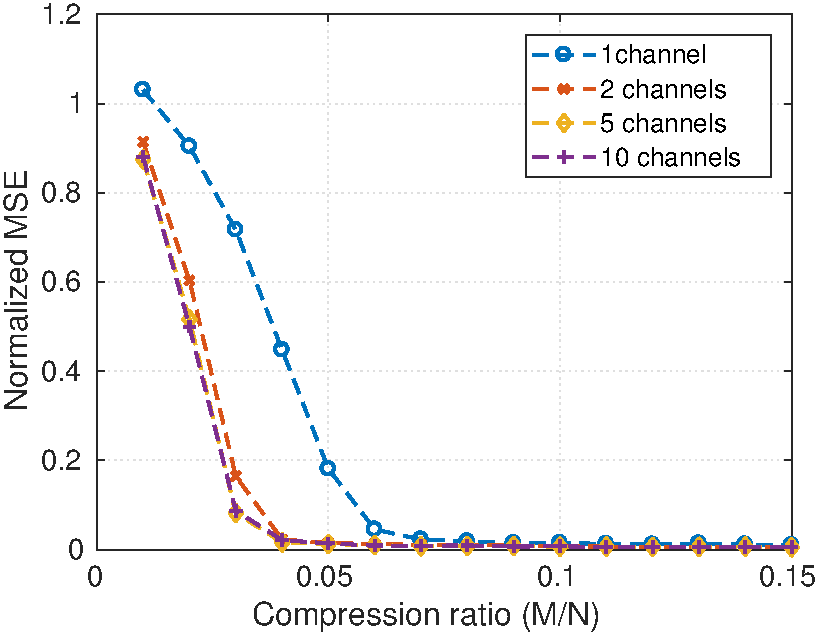
\includegraphics[width=\CohSubFigWidth]{Figures/NMSE_noiseless.pdf}}
\begin{figure}[htb]
	% Maximum length
	\hfill%
	\subcaptionbox{\label{fig_synth_US_nmse}}{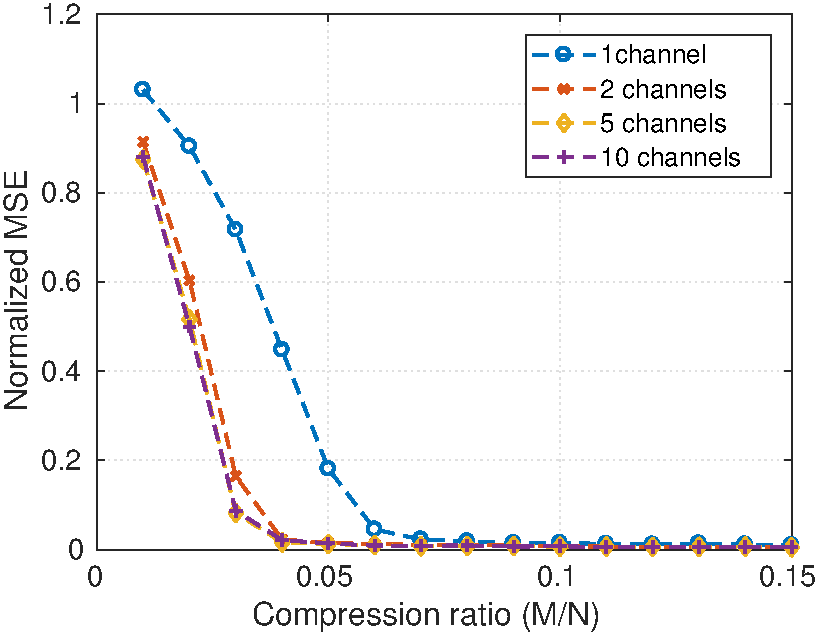
\includegraphics[height=\CohSubFigHeight]{Figures/NMSE_noiseless.pdf}}\hfill%
	\subcaptionbox{\label{fig_synth_US_nmse_2lambda}}{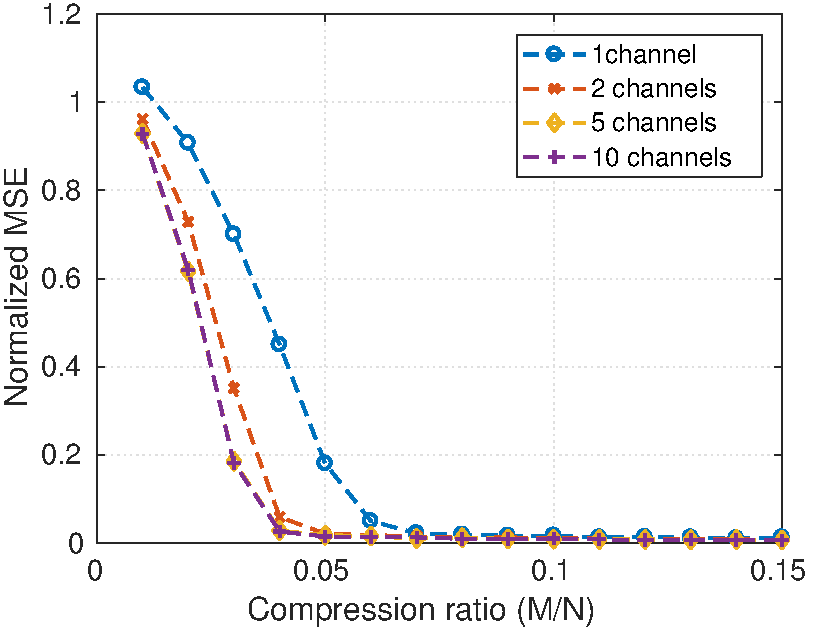
\includegraphics[height=\CohSubFigHeight]{Figures/NMSE_noiseless_2lambda.pdf}}\hfill%
	\caption{Normalized MSE for (a) $\Delta = $ \SI{0.31}{\milli\metre}~(one wavelength) and (b) $\Delta = $ \SI{0.62}{\milli\metre}~(two wavelengths) vs.\@ the compression ratio~($M/N$) for the proposed method for \num{1}-, \num{2}-, \num{5}- and \num{10}-channel scenarios. Signals parameters: $N=2000$, $F=31$, $K=20$.}
	\label{fig_synth_US}
\end{figure}
%%%%%%%%%%%% FIGURE %%%%%%%%%%%
\settoheight{\CohSubFigHeight}{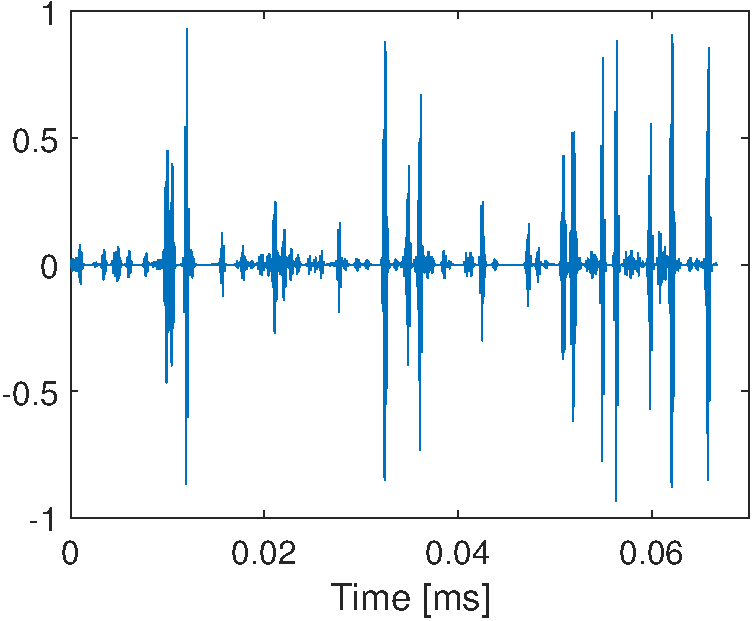
\includegraphics[width=\CohSubFigWidth]{Figures/res_1channel.pdf}}
\begin{figure*}[htb]
	% Maximum length
	\hfill%
	\subcaptionbox{\label{fig_channel_ref}}{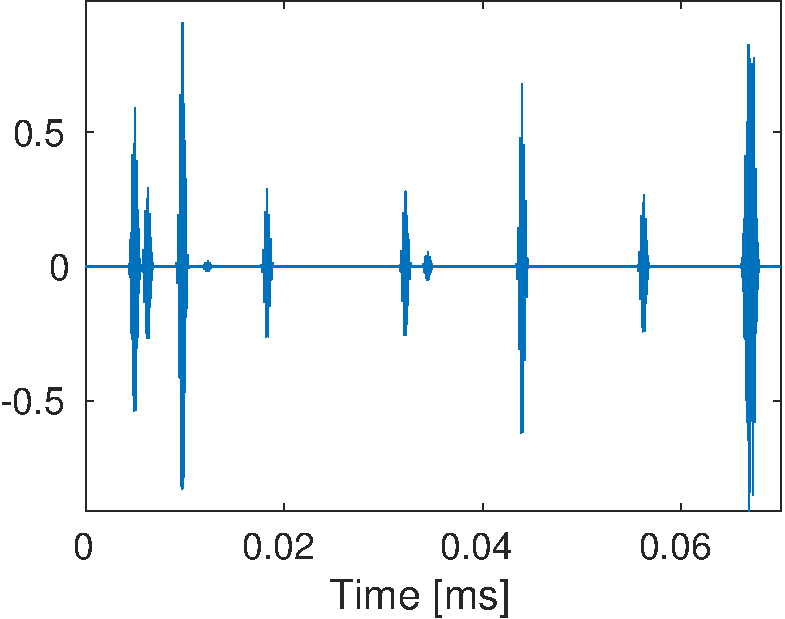
\includegraphics[height=\CohSubFigHeight]{Figures/channel_ref.pdf}}\hfill%
	\subcaptionbox{\label{fig_channel_noisy}}{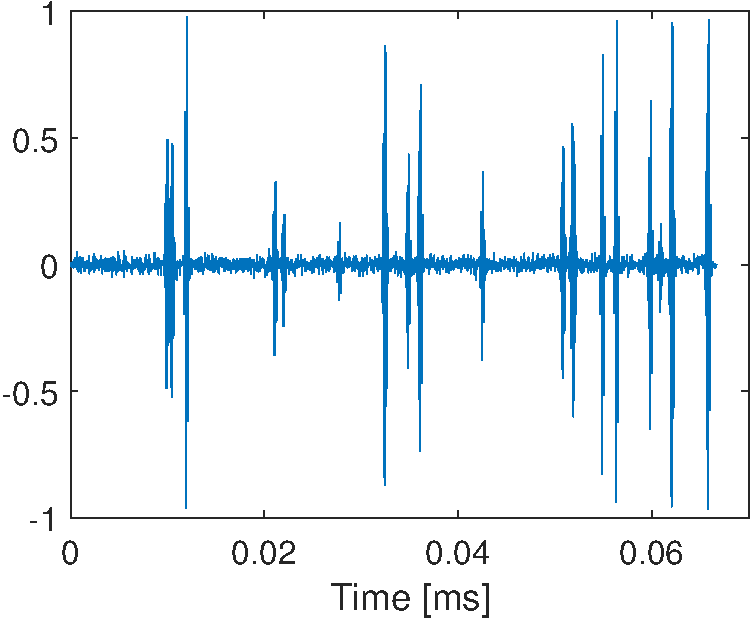
\includegraphics[height=\CohSubFigHeight]{Figures/channel_noisy.pdf}}\hfill%
	\subcaptionbox{\label{fig_res_1chan}}{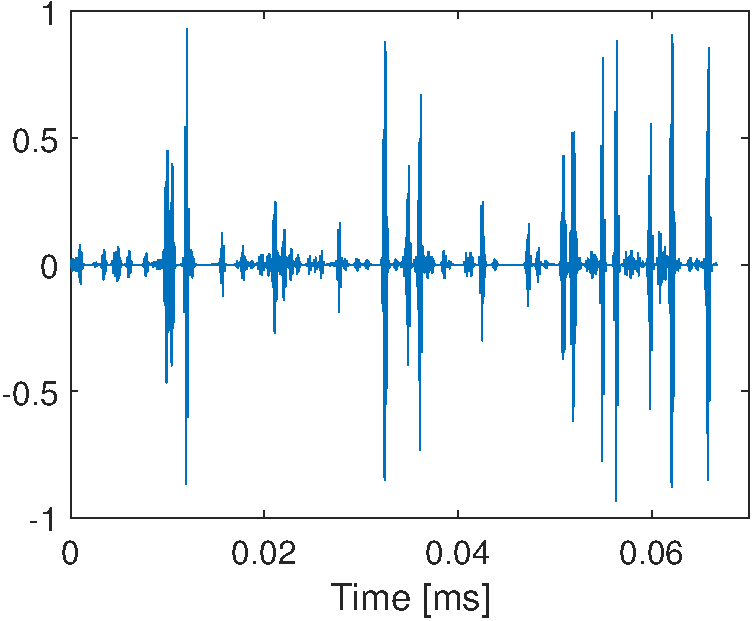
\includegraphics[height=\CohSubFigHeight]{Figures/res_1channel.pdf}}\hfill%
	\subcaptionbox{\label{fig_res_5chan}}{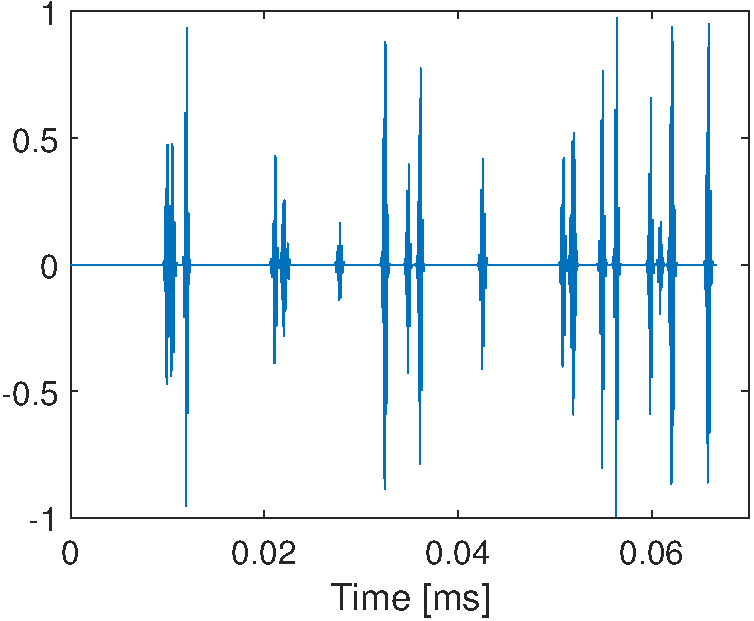
\includegraphics[height=\CohSubFigHeight]{Figures/res_5channels.pdf}}\hfill%
	\caption{(a) Original signal (b) Noisy signal~(SNR~=~\SI{30}{\decibel}) (c) Recovered estimate from $M$~=~\num{160} measurements in a \num{1}-channel scenario (d) Recovered estimate from $M$~=~\num{160} measurements in a \num{5}-channel scenario.}
	\label{fig_synth_noisy}
\end{figure*}

We consider a synthetic configuration with $K=$~\num{20} point-scatterers with random amplitudes and positions are generated. 
\num{10} sensors are considered, with an inter-sensor spacing of $\Delta$. Pulse-streams of length $N = 2000$ are simulated mimicking ultrasound plane-wave imaging with normal incidence~\cite{montaldo_uffc_2014}.
The considered pulse $h\left(t\right)$ is a convolution between a $2$-cycle square excitation signal and a Gaussian pulse~(\num{2.5} cycles, center frequency \SI{5.208}{\mega\hertz}, bandwidth \SI{67}{\percent}) which mimics the impulse response of ultrasound transducer elements. The sampling frequency $f_s$ is set to \SI{20.8}{\mega\hertz} which corresponds to four times the center frequency.

Fig.~\ref{fig_synth_US} displays the averaged results of a Monte-Carlo simulation over \num{1000} trials of the ADMM algorithm. 
Each trial was conducted by randomly generating the amplitudes and positions of the $K$ point-scatterers, the Gaussian \textit{i.i.d.} matrix $\mat{\Phi} \in \mathbb{R}^{M \times N}$ and by reconstructing the raw data $\vect{m}$ of one sensor from different values of $M/N$. single-channel as well as multi-channel scenarios are considered. 
For the multi-channel scenarios, prior knowledge on the support of the spike trains of \num{1}, \num{4} and \num{9} neighboring sensors of the sensor of interest are considered. 
Figure~\ref{fig_synth_US_nmse} and~\ref{fig_synth_US_nmse_2lambda} show the normalized mean squared error~(NMSE), calculated as $\| \vect{m} - \vect{m}^\star \|_2 / \| \vect{m}\|_2$, where $\vect{m}$ is the reference and $\vect{m}^\star$ the estimate, for two different inter-sensor spacings, namely \SI{0.31}{\milli\metre}~(one wavelength) and \SI{0.62}{\milli\metre}~(two wavelengths). 
Regarding the optimization algorithm, the maximum number of iterations is set to \num{1000} and $\epsilon = 0$. 
This experiment also demonstrates that considering a higher number of channels, which decreases the dimension of the subspace $S$~(Theorem 2), results in a better recovery. Indeed, Fig.~\ref{fig_synth_US_nmse} show that the 10- and 5-channel scenarios outperform the 2-channel one.

Figure~\ref{fig_synth_noisy} shows that the proposed algorithm is robust to small amount of noise~(SNR~=~\SI{30}{\decibel}). 
For this experiment, a small amount of Gaussian noise is added to the element raw-data of each sensor, leading to the signal displayed on Figure~\ref{fig_channel_noisy}. Figures~\ref{fig_res_1chan}~and ~\ref{fig_res_5chan} show the recovered signals for the \num{1}-channel and \num{5}-channels scenarios, respectively, for a number of measurements $M$~=~\num{160}. 
It can be seen that the signal recovered from the \num{5}-channel scenario is closer to the original signal than the one recovered from the \num{1}-channel scenario.
\subsection{Experimental non-destructive-evaluation signals}
\label{subsec_invivo_images}
An aluminum block containing side drilled holes located at different depths have been insonified with 1 plane wave~(normal incidence) using an open phased-array platform~(OEM-PA, Advanced OEM Solutions, Cincinnati, Ohio, USA), equipped with a linear probe~(Imasonic SAS, Voray-sur-l'Ognon, France) composed of \num{64} elements with \SI{0.93}{\milli\metre} pitch, working at \SI{5}{\mega\hertz} with \SI{100}{\percent} bandwidth. The sampling frequency has been set to \SI{50}{\mega\hertz} and the speed of sound in aluminum is \SI{6300}{\meter\per\second}. 
After acquisition, the element raw-data are imported on MATLAB and compressed using a Gaussian \textit{i.i.d.} matrix $\mat{\Phi} \in \mathbb{R}^{M \times N}$, with a compression ratio $M/N = 0.03$~(\SI{7.5}{\percent} of the Nyquist frequency). The pulse is approximated as a convolution between a \num{0.5}-cycle excitation signal and a \num{1}-cycle Gaussian-modulated sinusoidal impulse response. 
In the 1-channel scenario, all the channels are reconstructed in parallel. In the multi-channel scenario, a sequential reconstruction is achieved where each channel is recovered with prior knowledge on the support of the spike train corresponding to the neighbouring channel~(obtained from the previous reconstruction). The first channel is reconstructed from a compression ratio $M/N = 0.5$ in order to have a relevant first estimation of the support of the spike train. Concerning the optimization algorithm, the maximum number of iterations is set to \num{1000} and $\epsilon = 0.3 \| \vect{y} \|_2$. 
Once the raw data are reconstructed from compressed measurements, standard delay-and-sum beamforming~\cite{montaldo_uffc_2014} is applied to generate the radio-frequency image. The envelope is extracted through Hilbert transform and normalized to obtain the B-mode image. 
Figure~\ref{fig_carotid_ref} displays the reference B-mode image obtained with no compression and Fig.~\ref{fig_carotid_multcha} shows the recovered B-mode image in the multi-channel scenario. It shows that the multi-channel scenario leads to a nearly perfect reconstrucion, with a peak-signal-to-noise-ratio~(PSNR), calculated against the reference image, of \SI{28.3}{\decibel} while the \num{1}-channel scenario leads to significantly lower image quality~(PSNR~=~ \SI{25.5}{\decibel})\footnote{\scriptsize{\url{https://github.com/AdriBesson/ICASSP2018-pulse-streams}}}.
%%%%%%%%%%%% FIGURE %%%%%%%%%%%
\setlength{\CohSubFigWidth}{0.24\textwidth}
\settoheight{\CohSubFigHeight}{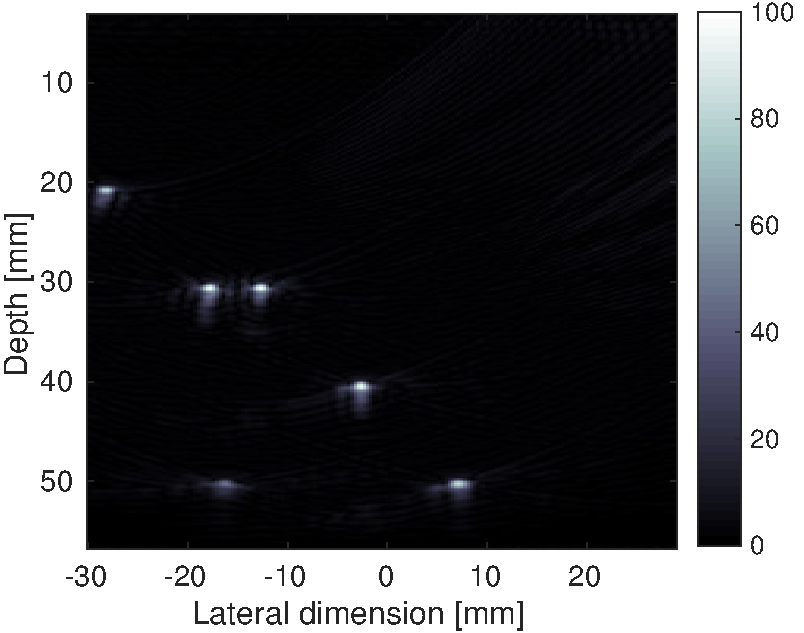
\includegraphics[width=\CohSubFigWidth]{Figures/cnd_ref.pdf}}
\begin{figure}[htb]
	% Maximum length
	\hfill%
	\subcaptionbox{\label{fig_carotid_ref}}{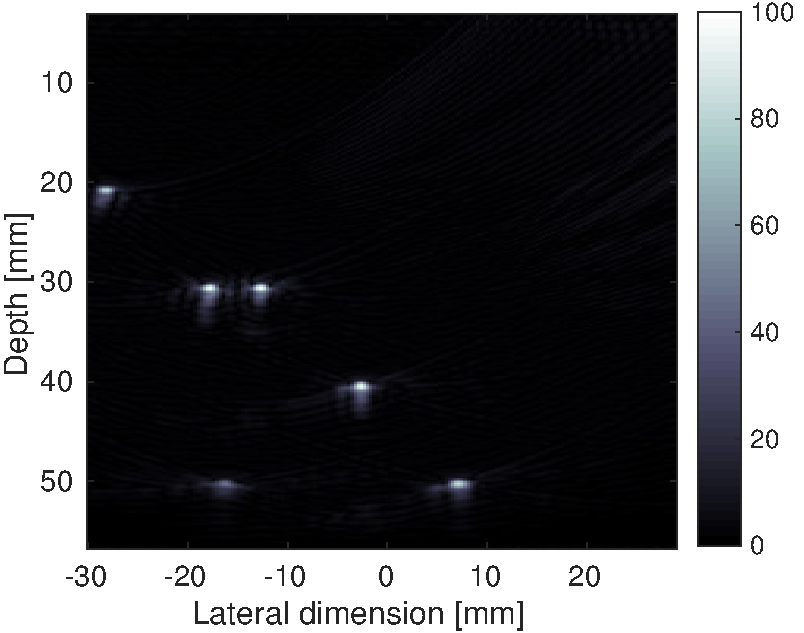
\includegraphics[height=\CohSubFigHeight]{Figures/cnd_ref.pdf}}\hfill%
	\subcaptionbox{\label{fig_carotid_multcha}}{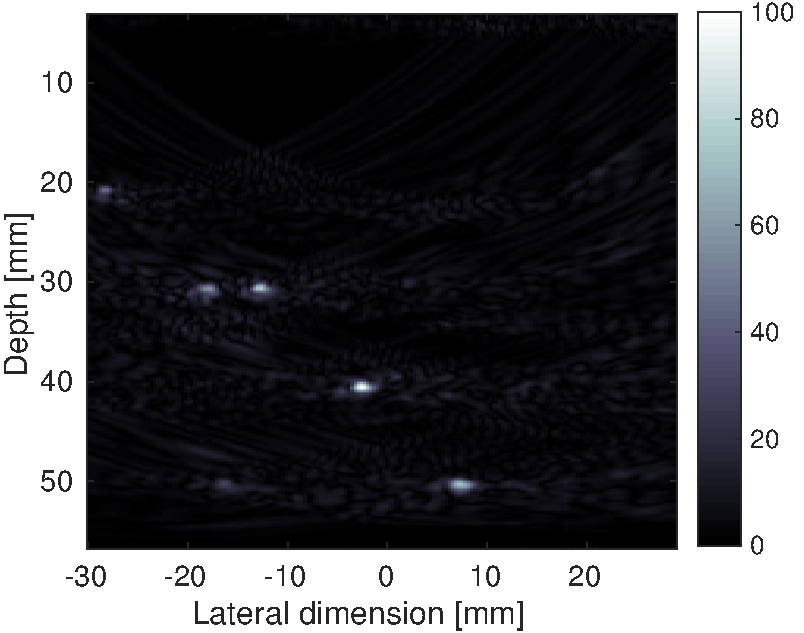
\includegraphics[height=\CohSubFigHeight]{Figures/cnd_rec_2channels.pdf}}\hfill%
	\caption{(a) Original B-mode image; (b) Recovered B-mode image from \SI{3}{\percent} measurements in a \num{2}-channels scenario~(PSNR~=~\SI{28.3}{\decibel}).}
	\label{fig_carotid}
\end{figure}
\subsection{Limitations of the proposed method}
\label{subsec_limitations}
The current method requires a perfect estimation of the support in order to perform efficient reconstructions which is very difficult to achieve in real scenarios. To address this problem, the non-uniform sparse framework~\cite{Khajehnejad_TSP_2011} will be explored in a future work. Another limitation of the current approach is the perfect knowledge of the pulse that can be tackled by exploring blind-deconvolution approaches~\cite{Hedge_TSP_2011, Demirli2001, Zhao_IUS_2016}.
\section{Conclusion}
\label{sec_concl}
We have presented an extension of the pulse-stream model coined as \textit{multi-channel pulse-stream model}. It accounts for the inter-sensor dependencies as an additional structure to the general pulse-stream model and enables us to quantitatively estimate the number of random projections necessary to sample such signals. We also suggest a reconstruction method based on $\ell_1$-minimization on the reduced signal support and illustrates its benefits on synthetic and experimental non-destructive-evaluation signals.





% if have a single appendix:
%\appendix[Proof of the Zonklar Equations]
% or
%\appendix  % for no appendix heading
% do not use \section anymore after \appendix, only \section*
% is possibly needed

% use appendices with more than one appendix
% then use \section to start each appendix
% you must declare a \section before using any
% \subsection or using \label (\appendices by itself
% starts a section numbered zero.)
%


% Can use something like this to put references on a page
% by themselves when using endfloat and the captionsoff option.



% trigger a \newpage just before the given reference
% number - used to balance the columns on the last page
% adjust value as needed - may need to be readjusted if
% the document is modified later
%\IEEEtriggeratref{8}
% The "triggered" command can be changed if desired:
%\IEEEtriggercmd{\enlargethispage{-5in}}

% references section

% can use a bibliography generated by BibTeX as a .bbl file
% BibTeX documentation can be easily obtained at:
% http://mirror.ctan.org/biblio/bibtex/contrib/doc/
% The IEEEtran BibTeX style support page is at:
% http://www.michaelshell.org/tex/ieeetran/bibtex/
\bibliographystyle{IEEEbib}
\bibliography{IEEEabrv,icassp_2018}

% biography section
% 
% If you have an EPS/PDF photo (graphicx package needed) extra braces are
% needed around the contents of the optional argument to biography to prevent
% the LaTeX parser from getting confused when it sees the complicated
% \includegraphics command within an optional argument. (You could create
% your own custom macro containing the \includegraphics command to make things
% simpler here.)
%\begin{IEEEbiography}[{\includegraphics[width=1in,height=1.25in,clip,keepaspectratio]{mshell}}]{Michael Shell}
% or if you just want to reserve a space for a photo:



% that's all folks
\end{document}


